\documentclass[12pt,a4paper]{article}
\usepackage{float}
\usepackage{commons/course}
\usepackage{xepersian}


\hidesolutions

\شروع{نوشتار}

\سربرگ{تمرین 4}{}{توزیع توام، توزیع شرطی و حاشیه‌ای، نامساوی های احتمالاتی}{گردآورندگان: امیررضا کاظمی، روزبه مشکین، پدرام خرسندی، آیدا رمضانی}

\section*{توزیع توام، توزیع شرطی و حاشیه‌ای، نامساوی های احتمالاتی
}


\مسئله{دست گرمی*}
صورت کلی مسئله 

\subsection*{الف}
صورت بخش اول 

\subsection*{ب}
صورت بخش دوم 

\subsection*{ج}
صورت بخش سوم

\حل{
	

می دانیم اگر $Y = g(X)$  و ریشه های معادله $y = g(x)$ به صورت $x_1 , x_2, ...$ باشند، داریم:
$$f_{Y}(y) = \sum \frac{f_{X}(x_{i})}{|g'(x)|}$$

\subsection*{الف}
$$Y = \ln(X) \implies X = e^{Y}$$
$$f_{Y}(y) = \frac{\frac{\theta}{x^{\theta + 1}}}{\frac{1}{x}} = \theta x^{-\theta} \implies f_{Y}(y) = \theta e ^ {-y\theta}$$
پس $Y$ از توزیع نمایی با پارامتر $\theta$ است و در نتبجه :
$$ E[y] = \frac{1}{\theta}, Var(y) = \frac{1}{\theta ^ 2} $$
\subsection*{ب}
$$f_{W}(w) = \frac{\lambda e^{-\lambda y}}{\frac{1}{2 \sqrt{y}}}, y = w^{2} \implies 2w\lambda e^{-\lambda w^{2}} \sim weibull(\alpha = 2 , \beta = \frac{1}{\lambda})$$

$$E[W] = \sqrt{\beta} \times \Gamma (1 + \frac{1}{\alpha}) = \frac{1}{\sqrt{\lambda}}\Gamma (\frac{3}{2})$$
$$Var[W] = \beta[\Gamma(1 + \frac{2}{\alpha}) - (\Gamma(1 + \frac{1}{\alpha})) ^ {2}] = \frac{1}{\lambda}[\Gamma(2) - (\Gamma(\frac{3}{2})) ^ {2}]$$
\subsection*{ج}
$$f_{X}(x) = \frac{\frac{1}{\sqrt{2\pi}}e^{\frac{-z^2}{2}}}{e^{z}} = \frac{1}{\sqrt{2\pi}}e^{-\frac{(\ln x) ^ 2}{2}} \sim lognormal(\mu = 0, \sigma ^ 2 = 1)$$
$$E[x] = exp(\mu + \frac{\sigma ^ 2}{2}) = e ^ {\frac{1}{2}}$$
$$Var[x] = [exp(\sigma ^ 2) - 1]exp(2\mu + \sigma ^ 2) = e^2 - e$$
\subsection*{د}
$$x = z ^ 2 \implies z_{1} = \sqrt{x}, z_{2} = -\sqrt{x}$$
$$f_{X}(x) = \sum \frac{\frac{1}{\sqrt{2\pi}}e ^ {\frac{-z_{i} ^ 2}{2}}}{2|z_{i}|} = 2 \times \frac{1}{2\sqrt{2\pi x}}e ^ {\frac{-x}{2}} = \frac{1}{\sqrt{2 \pi x}}x ^ {-\frac{1}{2}}e ^ {-\frac{x}{2}} \sim gamma(k = \frac{1}{2} , \theta = 2)$$
$$E[X] = k\theta  = 1$$
$$Var[X] = k\theta ^ 2 = 2$$
دقت کنید که به طور کلی نیازی به در نظر گرفتن ضرایب ثابت در توزیع ها وجود ندازد ، چرا که نهایتا جمع(انتگرال) تابع توزیع چگالی برابر یک خواهد بود.

}


\مسئله{دست گرمی ۲}

تعداد زیرمجموعه های k عضوی از مجموعه ی $\{1, 2, 3, ..., n\}$ را بیابید که هیچ دو عضوی از آن متوالی نباشند.


\حل{
	\subsection*{الف}
$$E[X] = \sum_{i = 1}^{\infty} i P(X = i)$$
$$ = P(X = 1)$$
$$ + P(X = 2) + P(X = 1)$$
$$ + P(X = 3) + P(X = 2) + P(X = 1)$$
$$ . . .$$
حالا اگر به صورت ستونی جمع بزنیم(یعنی حاصل جمع ستون ها را در نظر بگیریم) ، تساوی بالا به دست می آید.
\subsection*{ب}
می دانیم که
$$F_X(x) = P(X \leq x) \implies 1 - F_X(x) = P(X > x)$$
در نتیجه:
$$\int_{0}^{\infty} (1-F_X(x))\,dx = \int_0^\infty P(X> x) dx = \int_0^\infty \int_x^\infty f_X(y) dy dx$$
$$= \int_{0< x< y< \infty} f_X(y) d (x,y) = \int_0^\infty \int_0^y f_X(y) dx dy$$
از طرفی می دانیم:
$$\int_0^y f_X(y)\operatorname d x = f_X(y) \int_0^y 1\operatorname d x = y~f_X(y)$$
بنابراین:
$$\int_0^\infty P(X> x)dx = \int_0^\infty yf_X(y) dy = E(X \mid X\geq 0)P(X\geq 0) = E[X]$$ 
در صورتی که $X$ همواره مثبت باشد.


}

\مسئله{متغیر تصادفی های مستقل*}

توزیع \lr{Pareto}  با دو پارامتر $\alpha$ و $x_m$ مشخص می‌شود. می‌دانیم که $x_1$، $x_2$، ... و $x_n$ داده‌هایی رندوم از توزیع \lr{Pareto} با $\alpha  >2$ هستند. خصوصیات توزیع \lr{Pareto} داده‌هایمان در ادامه آورده شده است:
$$PDF:\ \frac{\alpha{x_m}^\alpha}{x^{\alpha+1}},\ \alpha>2,\ x_m>0,\ x\geq x_m$$
$$CDF:\ 1 - (\frac{x_m}{x})^\alpha$$
$$Mean:\ \frac{\alpha x_m}{\alpha - 1}$$
$$Variance:\ \frac{\alpha {x_m}^2}{(\alpha - 1)^2(\alpha - 2)}$$

\subsection*{الف}
با استفاده از تخمین‌گر \lr{MLE} پارامترهای $\alpha$ و $x_m$ را تخمین بزنید.

\subsection*{ب}
وضعیت \lr{unbiased} بودن و \lr{consistent} بودن تخمین‌گر \lr{MLE} برای $x_m$ را مشخص کنید. 
\\(راهنمایی: اگر n متغیر تصادفی \lr{iid} از توزیعی با $CDF:\ F$ باشند، مینیموم این متغیرها متغیر تصادفی‌ای با $CDF:\ 1-(1-F)^n$ است)

\حل{																																																				
	واقعه ی خرید روغن موتور را A 
و خرید لاستیک را B 
در نظر بگیرید.

در این صورت مقدار 
$P(A|B)$
را می خواهیم که از رابطه ی زیر بدست میاید:

$P(A|B) = \frac{P(A,B)}{P(B)} = \frac{\frac{20}{100}}{\frac{40}{100}} = 0.5$
}

\مسئله{توزیع توام}
\textbf{جدول
\lr{t}
در ادامه آمده است.}

اداره هواشناسی یک شهر، ۴ دستگاه سنجش آلودگی هوا را در یک منطقه قرار داده است. فرض کنید شاخص آلودگی هوا در این منطقه ثابت است اما این دستگاه‌ها دقیق نیستند و شاخص را با کمی نویز گزارش می‌دهند. در یک روز نسبتا آلوده، مقادیر گزارش شده توسط این ۴ دستگاه به شرح زیر است.
$$152, 148, 153, 153$$

\subsection*{الف}
با کمک داده‌های جمع آوری شده، یک بازه اطمینان ۹۵ درصد برای شاخص آلودگی هوا در آن ایستگاه ارائه دهید.

\subsection*{ب}
در صورتی که شاخص آلودگی هوا از ۱۵۰ بیشتر باشد، هوا در شرایط ناسالم برای تمامی گروه‌ها قرار می‌گیرد. عده‌ای از دانشمندان معتقدند که میانگین شاخص آلودگی ۱۵۰ بوده بنابراین هوای این منطقه ناسالم نیست، در حالی که عده‌ی دیگری معتقند میانگین شاخص آلودگی به طور معنی‌داری از ۱۵۰ بیشتر بوده و هوا ناسالم است. برای بررسی این افراد یک آزمون فرض طراحی کنید. فرض صفر و فرض دیگر این آزمون را بیان کرده و سپس مشخص کنید آیا با سطح اهمیت 
$0.05$
می‌توان فرض صفر را رد کرد یا خیر.

\subsection*{پ}
برای کاهش خطای نوع اول، باید سطح اهمیت را افزایش دهیم یا کاهش؟ برای کاهش خطای نوع دوم چه طور؟

\begin{figure}[H]
    \centering
    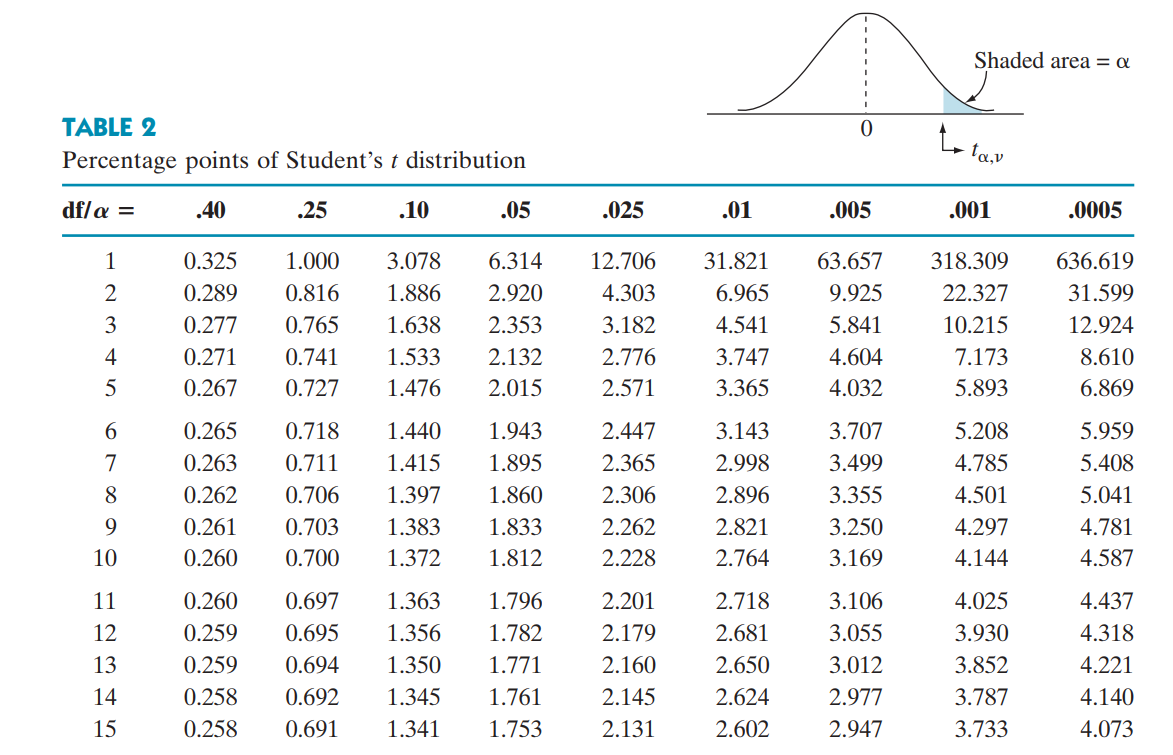
\includegraphics[width=7in,height = 5in]{tStudent}
\end{figure}

\حل{
	درست نیست ،به عنوان مثال در صورتی که:
$$S = \{1 , 2 , 3 , 4 \}$$
$$A = \{1 , 2 \} , B =  \{3 , 4 \} , C =  \{1 , 3 \} $$
داریم:
$$ P ( A \cap B ) = 0 = P ( A ) P ( B )  \Rightarrow  P ( A \cap B  | C)=0$$
$$ P (A|C)  P(B|C) = \frac{1}{4}  \Rightarrow P(A \cap B | C) \neq P(A | C) \times P(B | C)$$

}

\مسئله{شمارش تخم مرغی}

عمر چرخ یک ماشین مشخصی از یک توزیع نرمال با میانگین 34000 کیلومتر و انحراف از معیار 4000 کیلومتر پیروی می کند.

\subsection*{الف}
احتمال اینکه چرخ این ماشین بیش از 40000 کیلومتر عمر کند چقدر است؟
\subsection*{ب}
احتمال اینکه چرخ این ماشین بین 30000 تا 35000 کیلومتر عمر کند چقدر است؟
\subsection*{ج}
فرض کنید به ما گقته شده است که چرخ این ماشین تا الان 30000 کیلومتر عمر کرده است.احتمال اینکه 10000 کیلومتر دیگر عمر کند چقدر است.



\حل{
	توضیح کلی راه حل \\
 ابتدا بدیهیاتی که از سوال قابل استنتاج است را می‌نویسیم:
$$
X + Y = N    , \,   N  ~ Poisson(\lambda)  , \,    X|N = Bin(N, p)
$$
حال با استفاده از تعریف سوال را حل می‌کنیم:
$$
P(X = i, Y = j) = \Sigma_{n=0}^{\infty}P(X = i, Y = j | N = n) P(N = n)
$$
$$
 = P(X = i, Y = j| N = i + j) P(N = i + j)
$$
$$
 = P(X = i |  N = i + j) P(N = i + j)
$$
$$
= \dfrac{(i + j)! }{i! j!} p^i (1 - p) ^j e^{-\lambda} \dfrac{\lambda ^ {i + j}}{(i + j) !}
$$

$$
=  e^{-\lambda p}\dfrac{(\lambda p) ^ i}{i!} e^{-\lambda (1 - p)}\dfrac{(\lambda (1 - p)) ^ j}{j!}
$$



}

%%%%%%

\مسئله{جمع متغیرهای تصادفی*}

فزض کنید $f(x) = 0$ تابع توزیع یک متغیر تصادفی نرمال با میانگین $\mu$ و واریانس $\sigma ^ 2$ باشد.نشان دهید که $f''(x) = 0$ وقتی که $x$ برابر با مقادیر $\mu - \sigma$ و $\mu + \sigma$ باشد.

\حل{
	
\subsection*{الف}
اگر A عدد 1 را بنویسد و B به با احتمال $p$ به درستی عدد A را حدس بزند و با احتمال $1-p$ اشتباه حدس بزند، می‌توان امید ریاضی پول دریافتی توسط B را به شکل زیر محاسبه کرد:
$$
E(X_1) = 1\times p - 0.75(1 - p) = \frac{7}{4}p - \frac{3}{4}
$$


\subsection*{ب}
اگر A عدد 2 را بنویسد و B با احتمال $1-p$ درست حدس بزند و با احتمال $p$ اشتباه کند، می‌توان امید ریاضی پول دریافتی توسط B را به شکل زیر محاسبه کرد:
$$
E(X_2) = 2(1-p) - 0.75p = 2 - \frac{11}{4}p
$$

\subsection*{ج}
در این قسمت باید تابعِ
$
min(E(X_1), E(X_2)) = min(\frac{7}{4}p - \frac{3}{4}, 2 - \frac{11}{4}p)
$
را بررسی کنیم. اگر نمودار $E(X_1)$ و $E(X_2)$ که دو تابع خطی از $p$ هستند را رسم کنیم، می‌بینیم که مینیموم زمانی اتفاق می‌افتد که 
$$
\frac{7}{4}p - \frac{3}{4} = 2 - \frac{11}{4}p \Rightarrow p = \frac{11}{18} \Rightarrow \mathrm{maximied\,pool} = \frac{23}{72}
$$
}

\مسئله{جمع متغیرهای تصادفی گسسته}
صورت کلی مسئله 

\subsection*{الف}
صورت بخش اول 

\subsection*{ب}
صورت بخش دوم 

\subsection*{ج}
صورت بخش سوم

\حل{
	به طور کلی می‌توانیم تشخص دهیم که تابع توزیع Z تنها برای مقادیرِ
$$
R_Z = \{1, 2, 3, 4\}
$$
ناصفر است. \\
حالا تابع توزیع Z را در هر یک از این مقادیر محاسبه می‌کنیم.\\
برای 
$
z = 1
$
داریم:
\begin{align*}
P_Z(1) &= \sum\limits_{y \in R_y}^{} P_X(1 - y)P_Y(y) \\
&= P_X(1 - 1)P_Y(1) + P_X(1 - 2)P_Y(2) \\
&= \frac{1}{3} \times \frac{1}{3} + 0 \times \frac{2}{3}\\
&= \frac{1}{9}
\end{align*}
\\
برای 
$ z = 2 $
داریم:
\begin{align*}
P_Z(2) &= \sum\limits_{y \in R_Y}^{} P_X(2 - y)P_Y(y) \\
&= P_X(2 - 1)P_Y(1) + P_X(2 - 2)P_Y(2) \\
&= \frac{1}{3} \times \frac{1}{3} + \frac{1}{3}\times\frac{2}{3}\\
&= \frac{1}{3} 
\end{align*}
در حالت 
$
z = 3
$
داریم:
\begin{align*}
P_Z(3) &= \sum\limits_{y \in R_Y} P_X(3 - y)P_Y(y) \\
&= P_X(3 - 1)P_Y(1) + P_X(3 - 2)P_Y(2) \\
&= \frac{1}{3}\times\frac{1}{3} + \frac{1}{3}\times\frac{2}{3}\\
&= \frac{1}{3} 
\end{align*}

و در حالت 
$ z = 4 $
داریم:
\begin{align*}
P_Z(4) &= \sum\limits{y \in R_Y} P_X(4 - y)P_Y(y) \\
&= P_X(4 - 1)P_Y(1) + P_X(4 - 2)P_Y(2)\\
&= 0\times\frac{1}{4} + \frac{1}{3}\times\frac{2}{3}\\
&= \frac{2}{9}
\end{align*}
بنابراین، تابع توزیع متغیر تصادفی Z عبارتست از:
$$
P_Z(z) =
\begin{cases}
\frac{1}{9} &\quad z = 1\\
\frac{1}{3} &\quad z = 2\\
\frac{1}{3} &\quad z = 3\\
\frac{2}{9} &\quad z = 4\\
0 &\quad \text{otherwise}
\end{cases}
$$

}
%%%%%%



\مسئله{تابع توزیع متغیرهای تصادفی مستقل}
ثابت کنید متغیرهای
$ X_1 $
, ... ,
$ X_n $
مستقلند اگر و تنها اگر تابع توزیع توام آن‌ها به شکل زیر قابل بیان باشد.
\begin{center}
	$f( x_1, x_2, ..., x_n ) = \prod_{i=1}^n g_i(x_i)$
\end{center}
$ g_i $
تابعی مثبت است.

\حل{
	
متغیر تصادفی $X_k$ را تعداد توپ های متمایز پس از بزداشتن $k$ توپ از ظرف در نظر میگیریم. با دانستن $X_k$ احتمال برداشتن توپ جدید در مرتبه $k+1$ام  برابر با $\frac{n-X_k}{n}$ میباشد پس داریم\\
\centerline{$E(N_{k+1}\mid N_k)=N_k+\frac{n-N_k}{n}$}
بنابراین با توجه به این که $E(N_0) =0$ \\
\centerline{$\mathrm E(N_{k+1})=\mathrm E(N_k)+\frac{n-\mathrm E(N_k)}n=1+a_n\mathrm E(N_k)$}
به ازای هر $k \geq 0$\\
\centerline{$a_n=1-\frac1n$ => $\mathrm E(N_k)=\frac{1-a_n^k}{1-a_n}$}
و یا به طور معادل\\
\centerline{$\mathrm E(N_k)=n\,\frac{n^k-(n-1)^k}{n^{k}}=\sum\limits_{i=0}^{k-1}(-1)^{i}{k\choose i+1}\frac1{n^i}$}
}





\مسئله{نامساوی مارکوف}
فرض کنید متغیر تصادفی X از یک توزیع
$
Binomial(n, p)
$
می‌آید.
\subsection*{الف}
اگر
$
p < \alpha < 1
$
، با استفاده از نابرابری مارکوف، یک کران بالا برای 
$
P(X \ge \alpha n)
$
بیاید. 

\subsection*{ب}
مقدار عددی این کران را برای 
$
p = \frac{1}{2}
$
و
$
\alpha = \frac{3}{4}
$
بیابید.



\حل{
	با توجه به اینکه X یک متغیر تصادفی مثبت و 
$
E(X) = np
$
است، می‌توانیم از نابرابری مارکوف استفاده کنیم.

\subsection*{الف}
داریم:
$$
P(X \ge \alpha n) \le \frac{E(X)}{\alpha n} = \frac{pn}{\alpha n} = \frac{p}{\alpha}
$$

\subsection*{ب}
با جایگذاری 
$
p = \frac{1}{2}
$
و 
$
\alpha = \frac{3}{4}
$
داریم:
$$
P(X \ge \frac{3n}{4} ) \le \frac{2}{3}
$$

}





\مسئله{نامساوی چبیشف}

فرض کنید در یک پرواز، موتور های هواپیما به احتمال $1 - p$ خراب می شوند و احتمال خرابی هر موتور از موتور های دیگر مستقل است.اگر یک هواپیما برای پرواز نیاز داشته باشد تا بیشتر از نصف موتور هایش سالم باشند،به ازای چه مقادیری از $p$ یک هواپیما با 5 موتور را به یک هواپیما با 3 موتور ترجیح می دهید؟


\حل{
	\subsection*{الف}
می‌توانیم برای محاسبه کران بالا بنویسیم:
\begin{align*}
P(X \ge \alpha n) &= P(X - np \ge \alpha n - np) \\
&\le P(|X - np| \ge n \alpha - np) \\
&\le \frac{Var(X)}{(n\alpha - np)^2} \\
&= \frac{p(1 - p)}{n(\alpha - p)^2} \\
\end{align*}
\subsection*{ب}
با جایگذاری 
$
p = \frac{1}{2}
$
و 
$
\alpha = \frac{3}{4}
$
داریم:
$$
P(X \ge \frac{3n}{4}) \le \frac{4}{n}
$$

}



\مسئله{تراشه ها*}
حدود 2 درصد از تراشه‌های RAM تولید شده در یک کارخانه خراب است. علی به 50 عدد RAM سالم برای آزمایشگاهش نیاز دارد. علی باید چه تعداد تراشه RAM خریداری کند تا مطمئن باشد با احتمال حداقل 99 درصد، حداقل 49 تراشه سالم RAM دارد؟


\حل{
	\subsection*{الف}
$T_1$ و $T_2$ را به ترتیب زمان ملاقات دانشجوی اول و دوم در نظر میگیریم و زمان بین ورود دانشجوی اول و خروج دانشجوی دوم از رابطه $T = max(T_1,5) + T_2$ به دست می آید. مسئله را به دو حالت $T_1 < 5$ و $T_2 \geq 5$ تقسیم کرده و امید ریاضی $T$ به صورت $E[T] = pr(T_1 < 5)E[T|T_1 < 5] + pr(T_1 \geq 5)E[T|T_1 \geq 5]$ محاسبه میشود.\\

$$pr(T_1 < 5) = F(5) = 1 - e^{-\frac{5}{30}}$$

$$pr(T_1 \geq 5) = 1 - F(5) = e^{-\frac{5}{30}}$$

$$E[T|T_1 < 5] = E[T_2 + 5] = E[T_2] + 5 = 35$$

$$E[T|T_1 \geq 5] = E[T_2 + T_1 | T_1 \geq 5] = E[T_2] +  E[T_1| T_1 \geq 5]$$
 از آنجا که توزیع نمایی یک توزیع بی حافظه است این دانش اولیه که $T_1 \geq 5$ میباشد تاثیری بر مدت زمان باقیمانده از ملاقات ندارد و مدت زمان باقی مانده از همان توزیع نمایی امید ریاضی 30 پیروی میکند. بنابراین $E[T_1| T_1 \geq 5] = 30 +5 = 35$ و بنابراین\\
$$E[T|T_1 \geq 5] = 30 + 35 = 65$$
و با استفاده از رابطه $E[T]$ داریم \\
$$E[T] = (1 - e^{-\frac{5}{30}}) * 35 +  (e^{-\frac{5}{30}}) * 65 \approx 60.4 $$

\subsection*{ب}
متغیر تصادفی $X$ را زمان تاخیر دانشجوی دوم در نظر میگیریم. مانند قسمت قبل به ازای یک $x$ مشخص $E[T] = pr(T_1 < x)E[T|T_1 < x] + pr(T_1 \geq x)E[T|T_1 \geq x]$ و\\ 
$$pr(T_1 < x) = F(x) = 1 - e^{-\frac{x}{30}}$$
$$pr(T_1 \geq x) = 1 - F(x) = e^{-\frac{x}{30}}$$
$$E[T|T_1 < x] = E[T_2 + x] = E[T_2] + x = 30 + x$$
$$E[T|T_1 \geq 5] = E[T_2 + T_1 | T_1 \geq 5] = E[T_2] +  E[T_1] + x = 60 + x$$
$$\rightarrow E[T] = (1 - e^{-\frac{x}{30}}) * (30+x) +  (e^{-\frac{x}{30}}) * (60+x) = 30e^{-\frac{x}{30}} + 30 + x$$
با محاسبه این مقدار برای تمامی $x$ها به ازای احتمال آن ها امید ریاضی خواسته شده به دست می آید\\ 
$$\int_0^{+\infty} (30e^{-\frac{x}{30}} + 30 + x)\frac{1}{5}e^{-\frac{x}{5}}dx \approx 60.7 $$

}

\begin{flushleft}
	موفق باشید
\end{flushleft}



\پایان{نوشتار}
